% Created: 2019-12-10
% Plot participant data
% http://github.com/zhaobn/magic_stones

\documentclass{article}
\title{[Magic Stones] Report for Experiment 1}
\author{Bonan Zhao (b.zhao@ed.ac.uk)}

% Text formats: margin, font, spacing
\usepackage[margin=0.8in]{geometry}
\usepackage{charter}
\renewcommand{\baselinestretch}{1.3}

% Graphics
\usepackage{graphicx}
\usepackage{subcaption}
\graphicspath{{../figs/}}

\usepackage{amsmath}

\begin{document}
\maketitle

% Raw participant data
\section{Participant data}

\begin{figure}[h!]
	\centering
  \begin{subfigure}[t]{0.32\textwidth}
  	\centering
  	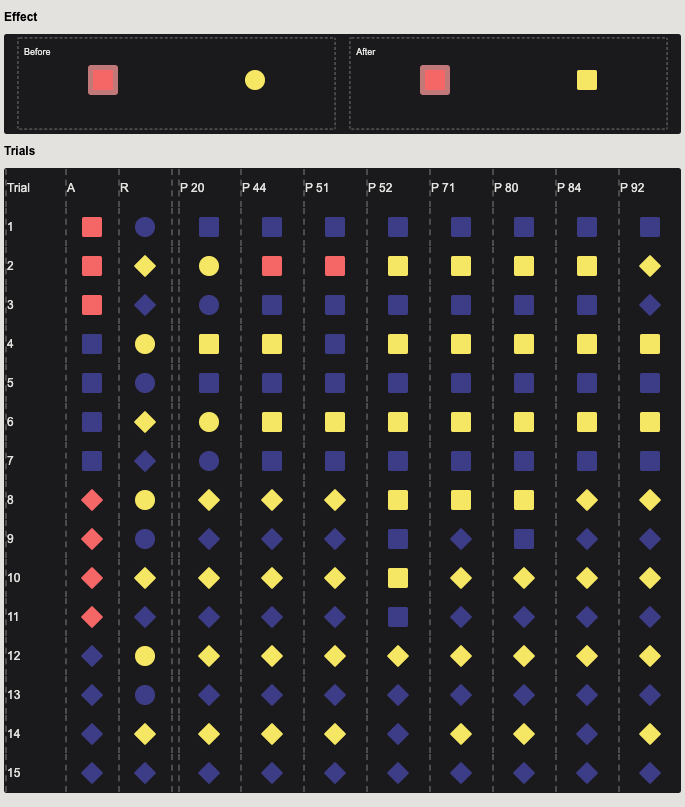
\includegraphics[width=\linewidth]{learn01} 
  	\caption{To the same shape} \label{fig:learn01}
  \end{subfigure}
  \hfill
  \begin{subfigure}[t]{0.32\textwidth}
  	\centering
  	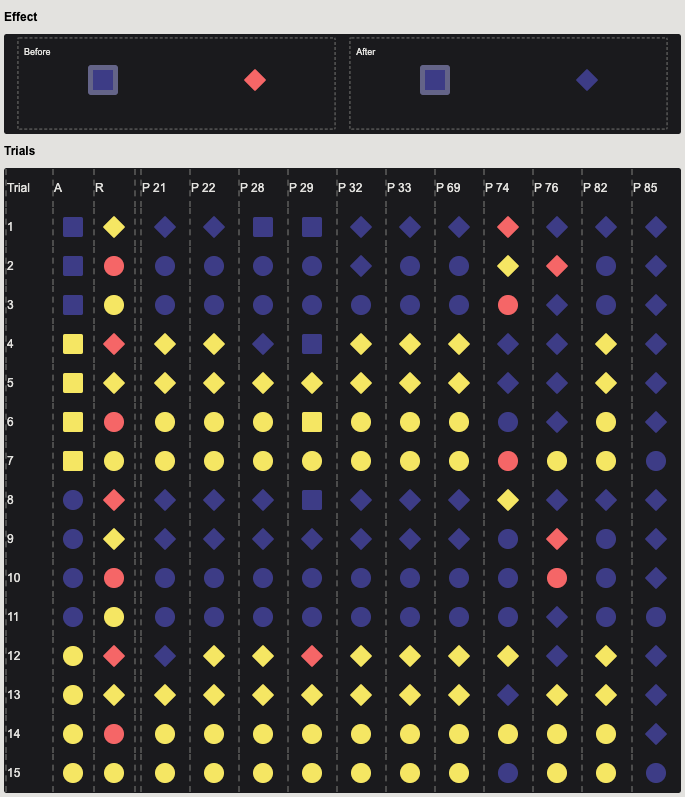
\includegraphics[width=\linewidth]{learn03} 
  	\caption{To the same color} \label{fig:learn03}
  \end{subfigure}
  \hfill
  \begin{subfigure}[t]{0.32\textwidth}
  	\centering
  	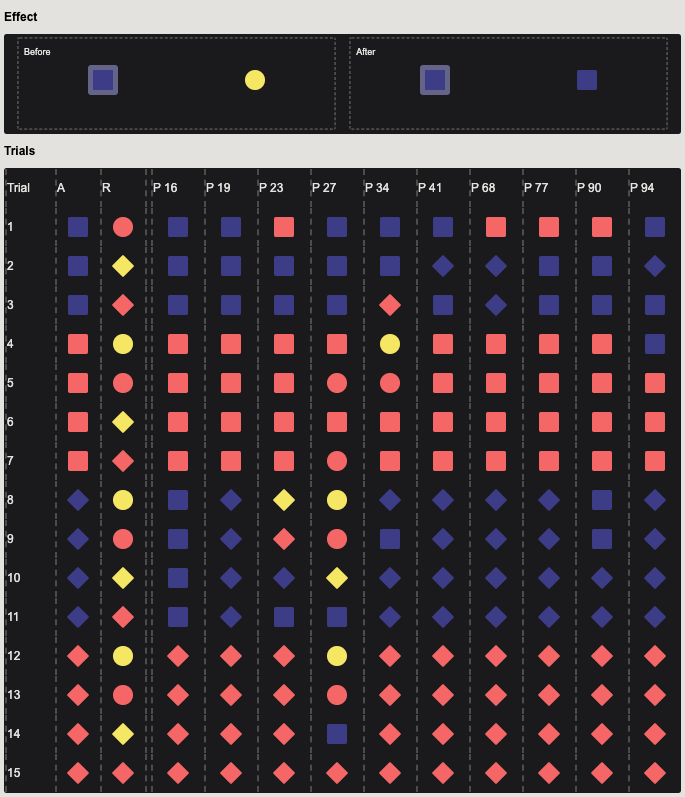
\includegraphics[width=\linewidth]{learn06} 
  	\caption{To the same object} \label{fig:learn06}
  \end{subfigure}

  \vspace{1em}
  \begin{subfigure}[t]{0.32\textwidth}
  	\centering
  	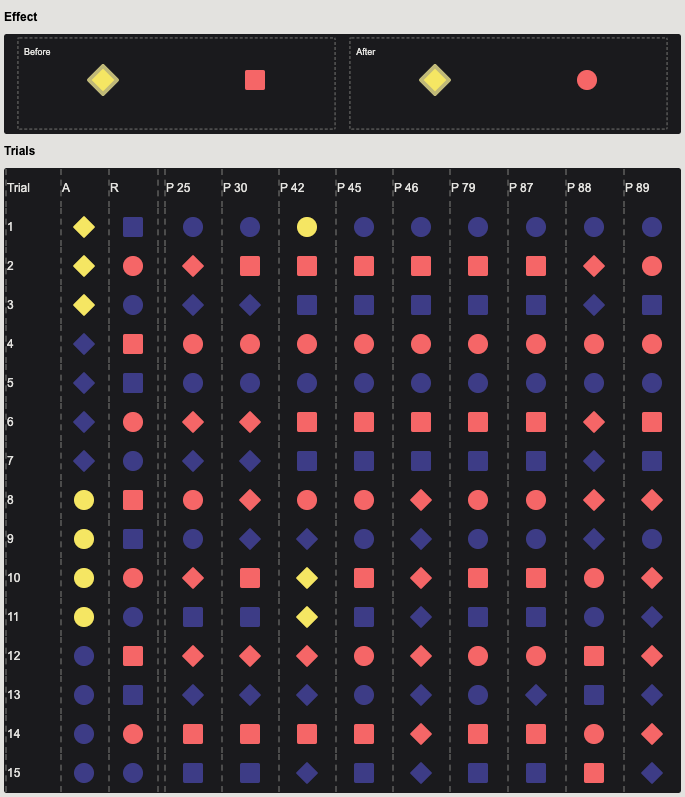
\includegraphics[width=\linewidth]{learn02} 
  	\caption{To a different shape} \label{fig:learn02}
  \end{subfigure}
  \hfill
  \begin{subfigure}[t]{0.32\textwidth}
  	\centering
  	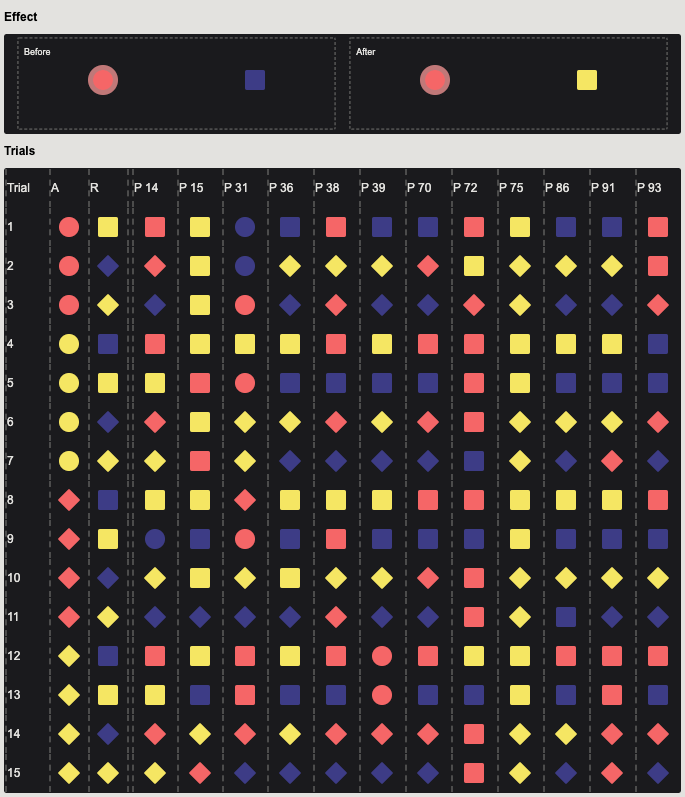
\includegraphics[width=\linewidth]{learn04} 
  	\caption{To a different color} \label{fig:learn04}
  \end{subfigure}
  \hfill
  \begin{subfigure}[t]{0.32\textwidth}
  	\centering
  	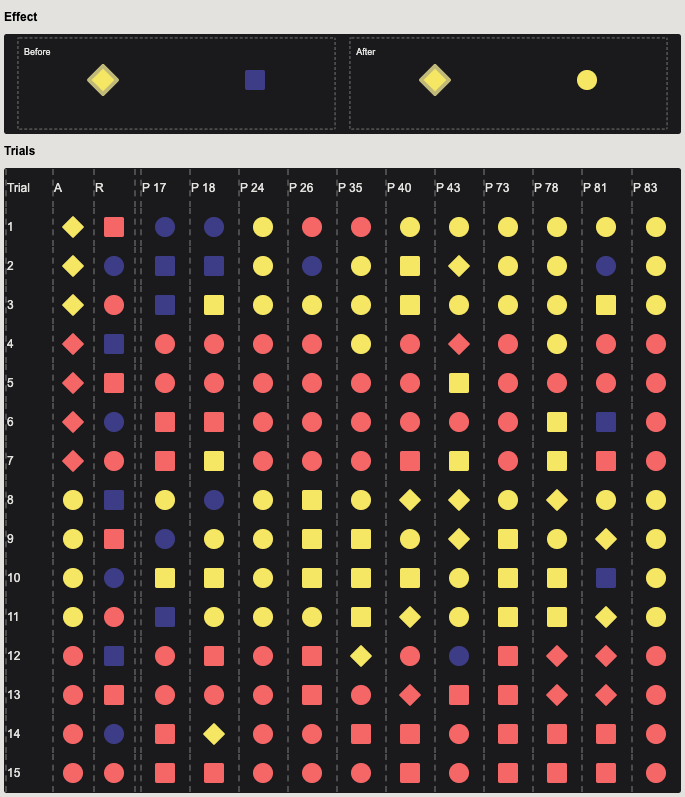
\includegraphics[width=\linewidth]{learn05} 
  	\caption{To a different object} \label{fig:learn05}
  \end{subfigure}
  \caption{Each figure is for one learning condition. 
  Each learning condition has 15 trials (15 rows).}
\end{figure}

\section{Stats}

\begin{itemize}
  \item Age: min 24, max 67, mean 41.1639, sd 11.1238 
  \item Gender: female 28 (45.9\%), male 33 (54.1\%)
  %\item Task duration (minutes): min 2.2068, max 10.0976, mean 4.8756, sd 1.8663
  %\item Self-report difficulty: min 0, max 10, mean 4.6557, sd 3.1564
\end{itemize}

\begin{table}[h!]
  \centering
  \begin{tabular}{c|l|c|c|c|c}
  Condition & Description & Count & Task dur. mean (min.) & S-Dfty. mean & Homogeneity \\
  \hline
  1        & To the same shape     & 8     & 5.1873 & 3.38 & 74.69\% \\
  2        & To a different shape  & 9     & 5.0942 & 3.45 & 57.10\% \\
  4        & To a different color  & 12    & 4.1504 & 5.17 & 34.06\% \\
  5        & To a different object* & 11   & 5.2803 & 5.09 & 36.53\% \\
  6        & To the same object    & 10    & 5.0351 & 3.00 & 65.50\% \\
  \hline
  Total    &                       & 61    & 4.8756 (sd 1.87) & 4.65 (sd 3.16) & \\
  \end{tabular}
  \caption{Basic stats per condition. S-Dfty.: Self-report difficulty.
  *: Same color + diff shape.}
  \label{table:conditions}
\end{table}

\subsubsection*{Homogeneity}

Homogeneity is defined as a scaled variance of selection frequency. Homogeneity $H$ for a trial $t_i$ for condition $C$ is calculated by

\[
var(\{\frac{n_{t_i}}{\sum_{i=1}^{15} n_{t_i}} | t_i \in C\})/var(M)
\]
where $M = \{1, \underbrace{0, ..., 0}_{14}, \}$



\begin{figure}[h!]
  \centering
  \begin{subfigure}[t]{0.32\textwidth}
    \centering
    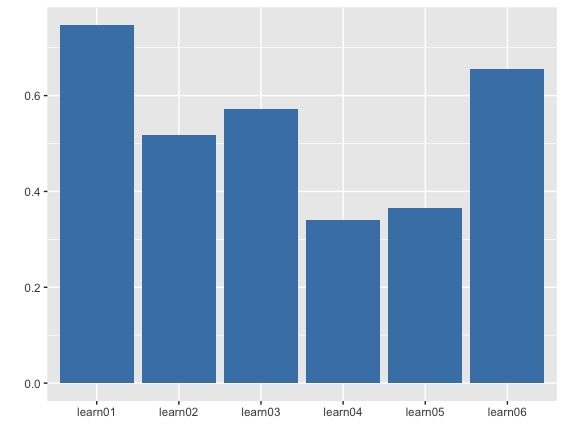
\includegraphics[width=\linewidth]{var_conditions} 
    \caption{Aggregated by conditions.}
  \end{subfigure}
  \hfill
  \begin{subfigure}[t]{0.32\textwidth}
    \centering
    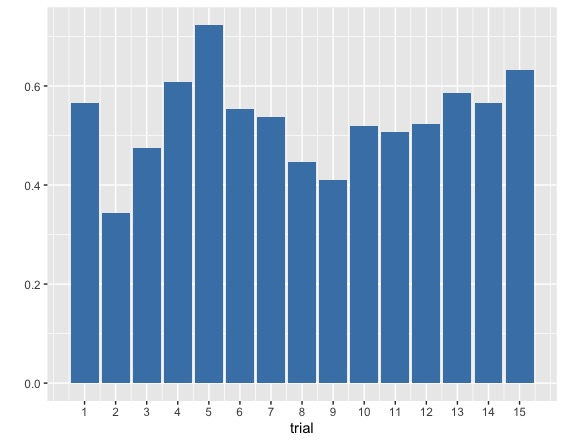
\includegraphics[width=\linewidth]{var_trials} 
    \caption{Aggregated by tasks.}
  \end{subfigure}
  \hfill
  \begin{subfigure}[t]{0.33\textwidth}
    \centering
    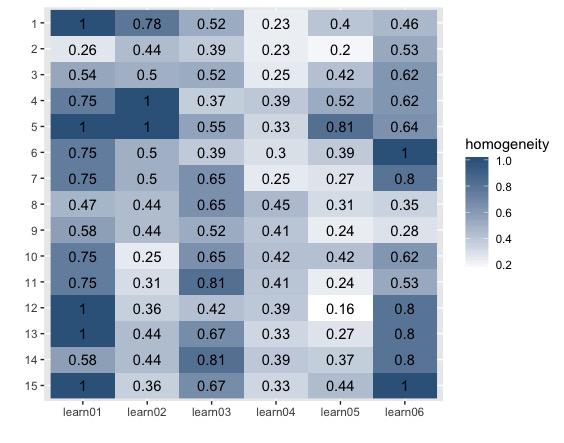
\includegraphics[width=\linewidth]{var_all} 
    \caption{Overall breakdown}
  \end{subfigure}
  \caption{Homogeneity.}
  \label{fig:var}
\end{figure}

\subsubsection*{``To the same xx'' V.S. ``To a different xx''}

Conditions 1, 3, and 6 can be classified as ``to the same xx'' group, where xx can be color, shape, or both (equivalent to the object), and conditions 2, 4, 5 can be classified as ``to a different xx'' group. Statistical test shows that compared to the ``to a different xx'' group, participant report the ``to the same xx'' group is significantly easier ($p<0.0001$), and make more homogeneous predictions ($p=0.0001$). However there is so significant difference for task duration between these two groups.


\section{Theories}

Recall the nine theories in previous notes, as listed in Table~\ref{functions}. Figure~\ref{fig:theory_comp} shows to what extent these nine theories predict the underlying rule or participant data separately.

Each cell is a summary of how well a theory predicts all the tasks for one condition, call it $A$ (for \emph{agreement}). For the ``code setup'' group, $A_C = N_C/15$ where $N_C$ is the number of theory predictions that agree with condition $C$'s underlying rule. When comparing with participant data, for each selection $s$ in the theory predictions $TP$ and participant selections $PP$, $A_C = (\sum_{i \in C}|P_{TH}(s_i) - P_{PP}(s_i)|)/15$.


\begin{table}
  \centering
  \begin{tabular}{rrrrrrrrrr}
    Arrow & $o \rightarrow o$ & $o \rightarrow c$ & $o \rightarrow s$ & $c \rightarrow o$ & $c \rightarrow c$ & $c \rightarrow s$ & $s \rightarrow o$ & $s \rightarrow c$ & $s \rightarrow s$ \\
    \hline \hline
    $|f|$ & 81  & 27  & 27  & 27  & 9   & 9   & 27  & 9   & 9   \\
    \hline
    Total &     &     &     &     &     &     &     &     & 225
  \end{tabular}
  \caption{Number of causal power functions each arrow combination produces. $o$: $object$, $c$: $color$, $s$:$shape$.}
  \label{functions}
\end{table}

\begin{figure}[h!]
  \centering
  \begin{subfigure}[t]{0.45\textwidth}
    \centering
    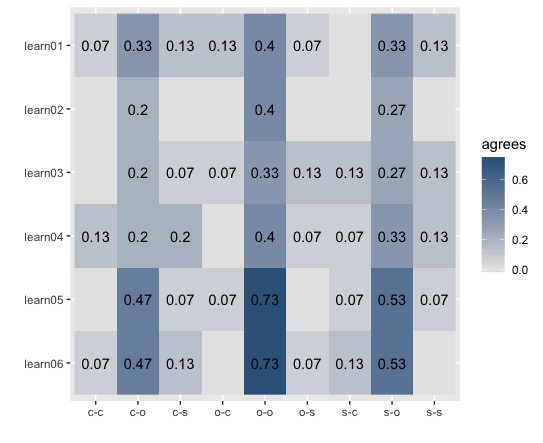
\includegraphics[width=\linewidth]{th_norm} 
    \caption{With code setup}
  \end{subfigure}
  \hfill
  \begin{subfigure}[t]{0.45\textwidth}
    \centering
    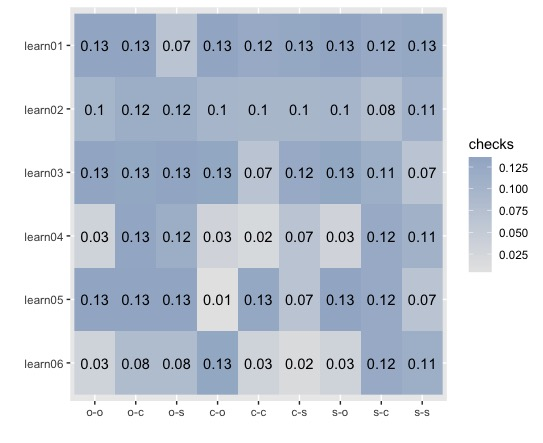
\includegraphics[width=\linewidth]{th_ppt} 
    \caption{With participant selections}
  \end{subfigure}
  \caption{Theory predictions versus data.}
  \label{fig:theory_comp}
\end{figure}


\end{document}


